\documentclass[oneside,zh]{nctuthesis}
\usepackage{enumitem}
\usepackage{times}
\usepackage{verbatim}
\usepackage{color}
\usepackage{url}
\usepackage{graphicx}
\usepackage{array}
\usepackage{pdfpages} % include inserted .pdf to page no.
\usepackage{wallpaper} % watermark

%for algorithm
%\usepackage{algorithmic}
\usepackage{amsmath}
\usepackage{amssymb}
\usepackage{graphics}
\usepackage{epsfig}

%for subfigure
\usepackage{subcaption}
% Format the refs
\usepackage[square,numbers]{natbib}

\usepackage[hidelinks]{hyperref}

% For Cross ref
\usepackage{xr}


% For the tree
\usepackage{tikz}
\usepackage{tikz-qtree}

% For code display
\usepackage{listings}

% For the APA table
\usepackage{adjustbox}
\usepackage{multirow,booktabs,setspace,caption}
\usepackage{rotating}
\usepackage{dcolumn}
\newcolumntype{z}{D{.}{.}{3}} % for decimal dot alignment

% For hyperlink
\usepackage{hyperref}

% For barchart
\usepackage{pgfplots}
\pgfplotsset{compat=1.12}

% For setting counters of figure and table
\usepackage{chngcntr}

% Using the tex-text mapping for ligatures etc.
\defaultfontfeatures{Mapping=tex-text}

% Set the default fonts
\setmainfont{Times New Roman}
\setCJKmainfont{標楷體} %modify for overleaf service

% Your information goes here
% author Po-Hao Huang [https://github.com/Po-haoHuang]

% ----------------------------------------------------------------------------
% "THE CHOCOLATE-WARE LICENSE":
% Tz-Huan Huang wrote this file. As long as you retain this notice you
% can do whatever you want with this stuff. If we meet some day, and you think
% this stuff is worth it, you can buy me a chocolate in return Tz-Huan Huang
% ----------------------------------------------------------------------------

% Syntax: \var{English}{Chinese}

%改動這邊並沒有用 因為封面那些都是pdf檔案 請自己改pdf檔

% \university{National Chiao Tung University}{國立交通大學}
% \college{College of Computer Science}{資訊學院}
% \institute{Institute of Computer Science and Engineering}{資訊科學與工程研究所}
% \title{Test}{測試}
%\author{englishName}{名字}
%\studentid{123456}
%\advisor{AAA, Ph.D.}{教授名字\ 教授}
% \defenseyear{2016}{105}
% \defensemonth{July}{7}
% \defenseday{1}


\begin{document}

% 論文浮水印 如需浮水印時取消此行註解
 % 論文浮水印
\CenterWallPaper{0.3}{pdfs/logo.pdf}
\setlength{\wpXoffset}{0 cm}
\setlength{\wpYoffset}{0 cm}


\hypersetup{pageanchor=false}

\frontmatter
\pagenumbering{gobble}

% 此處不自動產生交大封面改採插入pdf封面故註解
% \makecover

%以插入pdf檔方式加入封面及書名頁
\includepdf[pages={1}]{pdfs/cover.pdf}
\includepdf[pages={1}]{pdfs/first_page.pdf}



%插入論文審定書 著作權審定書等等

%\addcontentsline{toc}{chapter}{中文論文口試委員會審定書}
%\includepdf[pages={1}, pagecommand={}]{pdfs/ch.pdf}
%\addcontentsline{toc}{chapter}{Thesis Certificate}
%\includepdf[pages={1}, pagecommand={}]{pdfs/en.pdf}
%\addcontentsline{toc}{chapter}{論文著作權授權書}
%\includepdf[pages={1}, pagecommand={}]{pdfs/copyright.pdf}

% 開始編羅馬數字頁碼
\clearpages
\setcounter{page}{1}
\hypersetup{pageanchor=true}
\pagenumbering{roman}
\phantomsection
% 摘要 致謝
\begin{abstractzh}
\hfill\break

\begin{center}

\Large{中文論文題目}
\end{center}
\hfill\break
研究生: 姓名 $\hfill$指導教授:施仁忠 $\;$ 教授
%\begin{flushright}共指 $\;$ 教授\end{flushright}





\hfill\break

\begin{center}
國立交通大學多媒體工程研究所 \\

\hfill\break
摘\hspace{2cm}要\\
\end{center}


\hfill\break

中文摘要內容

\end{abstractzh}



\begin{abstracten}
%\hfill\break

\begin{center}
\Large{English thesis title}
\end{center}
\hfill\break

Student: name $\hfill$ Advisor: Prof. Zen-Chung Shih
%\begin{flushright}Prof. xxx\end{flushright}

\bigskip

\begin{center}
Institute of Multimedia Engineering\\
National Chiao-Tung University\\
\bigskip

ABSTRACT
\end{center}

\bigskip

English abstract.

\end{abstracten}

% 自行決定是否需英文摘要
\begin{acknowledgementsen}
\begin{center}
\bfseries
\LARGE{Acknowledgements}
\end{center}
\bigskip
\bigskip
CGLab Thanks You


\end{acknowledgementsen}



% % Table of Content
\clearpages
\tableofcontents

% % List of Figures
\clearpages
\listoffigures

% % List of Tables
\clearpages
\listoftables

\mainmatter
% tables and figures counter within chapter
%This create format such as Figure 1.1 
\counterwithin{table}{chapter}
\counterwithin{figure}{chapter}

% Your thesis goes here
\chapter{ Introduction}
\label{c:intro}

A subfigure example is shown in Figure \ref{i:style_set}.
\begin{figure}[!ht]
\centering
    \begin{subfigure}[b]{0.5\textwidth}
        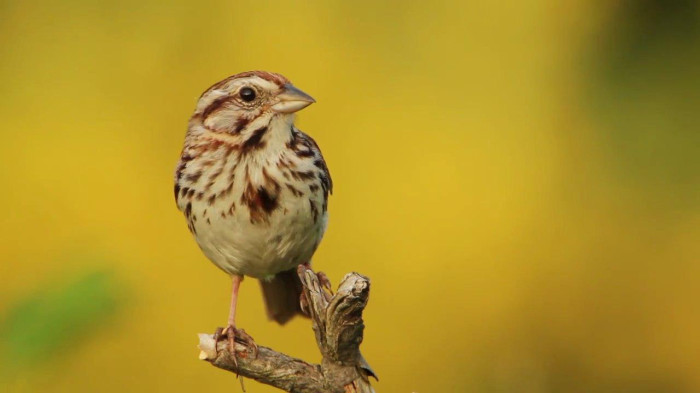
\includegraphics[width=\textwidth]{images/content_img}
        \caption{}
        \label{i:content}
    \end{subfigure}
    \begin{subfigure}[b]{0.4\textwidth}
        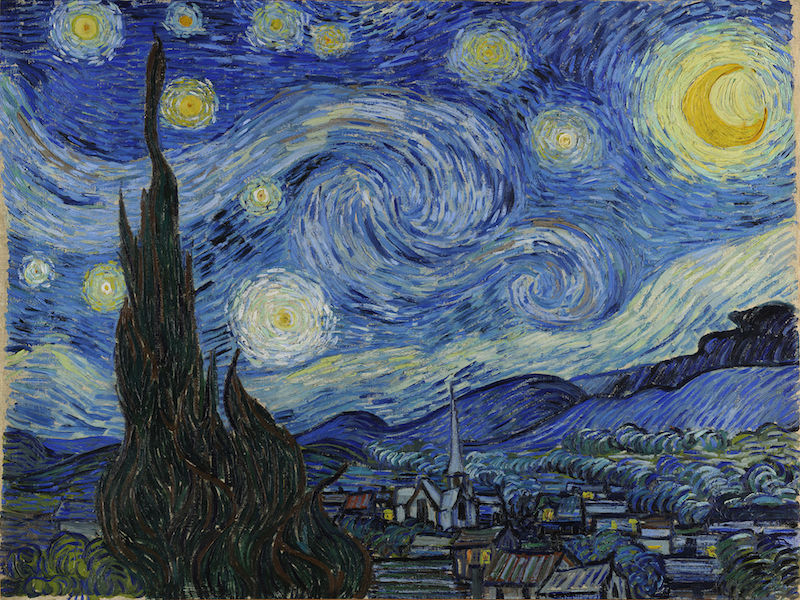
\includegraphics[width=\textwidth]{images/starry-night}
        \caption{}
        \label{i:style}
    \end{subfigure}
    \newline
    \begin{subfigure}[b]{0.5\textwidth}
        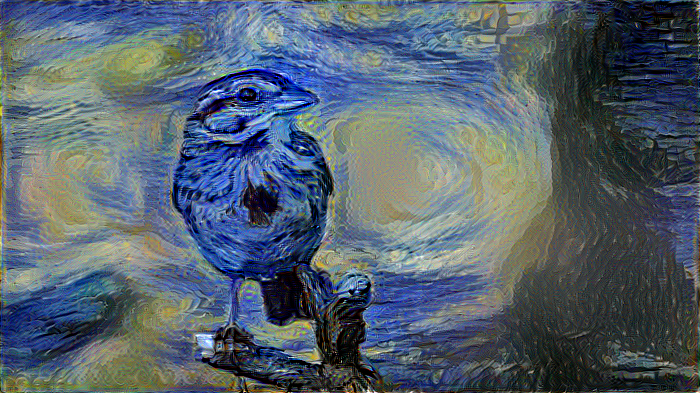
\includegraphics[width=\textwidth]{images/stylized_img}
        \caption{}
        \label{i:stylized}
    \end{subfigure}
\caption{blah blah blah.}\label{i:style_set}
\end{figure}


 A citation example \cite{styleVideo} 


\chapter{Related Works}

\section{sectionName}

\begin{figure}[!ht]
\centering
    \begin{subfigure}[b]{0.6\textwidth}
        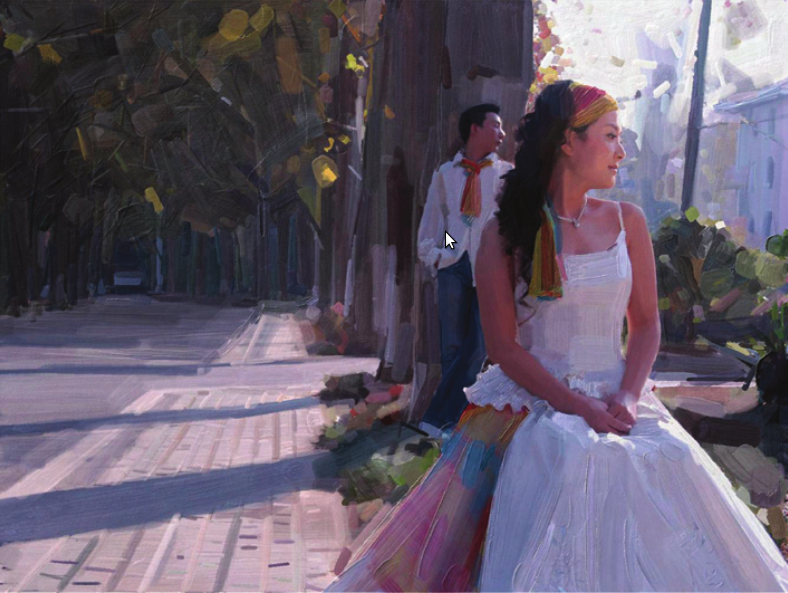
\includegraphics[width=\textwidth]{images/related/imageparse}
        \caption{}
    \end{subfigure}
    \begin{subfigure}[b]{0.33\textwidth}
        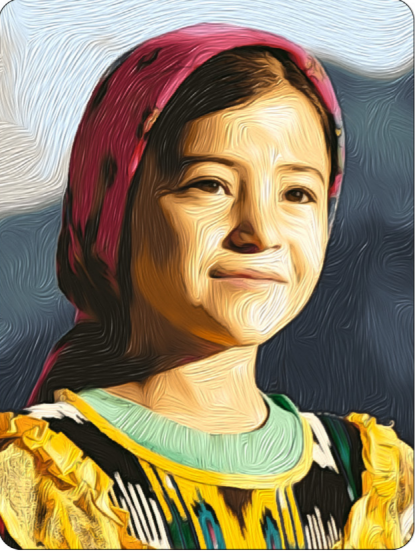
\includegraphics[width=\textwidth]{images/related/oilpaint}
        \caption{}
    \end{subfigure}
\caption{image descriptions \cite{Youtube}.}
\label{i:imageParse2Oil}
\end{figure}
\chapter{Method}
\section{sectionName}
好想畢業

\subsection{subsectionName}
An equation example is defined as
\begin{equation}
\sigma(x_{i}) =\frac{exp(x_{i})}{\sum_{k=1}^{K}exp(x_{k})} \, for \, i=1,...,K
\end{equation}


An algorithm example is as follows:
\begin{algorithm}[!ht]
  \caption{Algorithm title}
  \begin{algorithmic}[1]
    \Require
        $G$: Segmentation;
    \Ensure
        $C$: Cluster map;
    
    \State Initialization:  Let visited map $V$ and cluster map $C$ be $h x w$ zero arrays;
    \While {$V$ is not all visited}
        \State Push the first non-visited point $s$ into $Q$
        \While {$Q$ is not empty}
            \State $p$=$Q$.pop()

        \EndWhile
    \EndWhile

  \end{algorithmic}
\label{alg:algorithm_label}
\end{algorithm}


\chapter{Results}
\label{c:experiment}

%\section{描述性統計}
本研究各變數實驗結果之描述性統計(個數、最小值、最大值、平均與標準差)如表~\ref{4-0}。

\input{tables/4-0.tex}


%\section{實驗結果分析}

如表~\ref{4-4},以雙獨立樣本t檢定檢驗...

\input{tables/4-4.tex}





如表~\ref{4-9}所示...

\input{tables/4-9.tex}

\chapter{Conclusion and Discussion}
\label{c:conclusion}





\backmatter

\clearpages
\phantomsection
\addcontentsline{toc}{chapter}{\bibname}
%You can change the citation format here (Natbib bibliography styles), if you want to use bibtex style 
%Get more Natbib bibliography styles: https://www.sharelatex.com/learn/Natbib_bibliography_styles
%Sorting according to the last name of first author.
\bibliographystyle{abbrvnat}

%Where the bibliography will be printed
\bibliography{thesis}
\@startappendix

% 交大圖書館規定附錄在參考文獻之後
%\input{chapters/otherbib}
\end{document}
